\documentclass[12pt,a4paper]{article}
\usepackage[utf8]{inputenc}
\usepackage[T1]{fontenc}
\usepackage{amsmath}
\usepackage{amsfonts}
\usepackage{amssymb}
\usepackage{makeidx}
\usepackage{graphicx}
\usepackage{color}
\usepackage{multirow}
\usepackage{listings}
\definecolor{editorGray}{rgb}{0.95, 0.95, 0.95}
\definecolor{editorOcher}{rgb}{1, 0.5, 0} % #FF7F00 -> rgb(239, 169, 0)
\definecolor{editorGreen}{rgb}{0, 0.5, 0} % #007C00 -> rgb(0, 124, 0)
\usepackage{upquote}
\usepackage{listings}
\lstdefinelanguage{JavaScript}{
	morekeywords={typeof, new, true, false, catch, function, return, null, catch, switch, var, if, in, while, do, else, case, break},
	morecomment=[s]{/*}{*/},
	morecomment=[l]//,
	morestring=[b]",
	morestring=[b]'
}

\lstdefinelanguage{HTML5}{
	language=html,
	sensitive=true, 
	alsoletter={<>=-},
	otherkeywords={
		% HTML tags
		<html>, <head>, <title>, </title>, <meta, />, </head>, <body>,
		<canvas, \/canvas>, <script>, </script>, </body>, </html>, <!, html>, <style>, </style>, ><
	},  
	ndkeywords={
		% General
		=,
		% HTML attributes
		charset=, id=, width=, height=,
		% CSS properties
		border:, transform:, -moz-transform:, transition-duration:, transition-property:, transition-timing-function:
	},  
	morecomment=[s]{<!--}{-->},
	tag=[s]
}

\lstset{%
	% Basic design
	backgroundcolor=\color{editorGray},
	basicstyle={\small\ttfamily},   
	frame=l,
	% Line numbers
	xleftmargin={0.75cm},
	numbers=left,
	stepnumber=1,
	firstnumber=1,
	numberfirstline=true,
	% Code design   
	keywordstyle=\color{blue}\bfseries,
	commentstyle=\color{darkgray}\ttfamily,
	ndkeywordstyle=\color{editorGreen}\bfseries,
	stringstyle=\color{editorOcher},
	% Code
	language=HTML5,
	alsolanguage=JavaScript,
	alsodigit={.:;},
	tabsize=2,
	showtabs=false,
	showspaces=false,
	showstringspaces=false,
	extendedchars=true,
	breaklines=true,        
	% Support for German umlauts
	literate=%
	{Ö}{{\"O}}1
	{Ä}{{\"A}}1
	{Ü}{{\"U}}1
	{ß}{{\ss}}1
	{ü}{{\"u}}1
	{ä}{{\"a}}1
	{ö}{{\"o}}1
}

\usepackage[linesnumbered,ruled,vlined]{algorithm2e}
\newcommand\mycommfont[1]{\footnotesize\ttfamily\textcolor{blue}{#1}}
\SetCommentSty{mycommfont}

\begin{document}
	\textbf{ \centering \Huge Digital Innovation One: HTML Web Developer} % article
	%\chapter{Curso em vídeo - Excel} % report
	
	Aprenda a programar páginas de internet e desenvolver websites utilizando HTML, CSS e JavaScript para iniciar sua trajetória profissional em desenvolvimento web front-end.
	
	\section{Bem vindo à DIO}
	
	Seja bem vindo à Digital Inoovation ne, o maior ecossistema open education em desenvolvimento  de software da América Latina. VOcê vai comear agora uma jornada para criar o seu currículo com portfólio de projetos inovadores e acelerar a sua carreira para conquistar grandes oportunidades.
	
	\subsection{O que é a Digital Innovation One?}
	
	\subsection{Por que a carreira em desenvolvimento de software tem um futuro muito promissor?}
	
	\textbf{Digital transformation}. Porque para ser competitiva as empresas precisam gerar valor contínuo para seus clientes, parceiros e sociedade. A tecnologia habilita isso.
	
	\subsection{Alinhando a sua mentalidade a dos desenvolvedores de software de alto desempenho}
	
	\textbf{Soft skill} (atitude, protagonismo, disciplina, criatividade, colaboração e curiosidade) e \textbf{hard skill}.
	
	\subsection{Conhecendo a plataforma da Digital Innovation One}
	
	\subsection{Como tirar dúvidas técnicas sobre aulas, desafios e projetos?}
	
	\subsection{10 dicas para ser contratado por uma empresa inovadora de tecnologia}
	
	\textbf{	Características dos aprovados:}
	\begin{itemize}
		\item Repositório de projetos alinhado ao currículo;
		\item Artigos publicados e construção de conhecimento público na internet;
		Integração colaborativa a uma comunidade de desenvolvimento de software;
		\item Sonho grande e ambição para crescer profissionalmente;
		\item Utilização das principais comunidades e sites internacionais para suas pesquisas (stackoverflow);
		\item Graduação na área de exatas;
		\item Evidências de contatos com as novas tecnologias: Cloud, BigData, IA, reconhecimento de voz, mobilidade etc;
		\item Conhecimento em metodologias ágeis, devops e ux;
		\item Contas em provedores cloud e ferramentas online para devs;
		\item Evidências de aprendizagem contínua através da internet.
	\end{itemize}

	\textbf{Características dos não aprovados:}
	\begin{itemize}
		\item Não tem projetos e portfólio para apresentar;
		\item Não conhece e nunca praticou as novas tecnologias;
		\item Não está conectado a nenhuma comunidade de aprendizagem seja físico ou digital;
		\item Não apresenta elementos de colaboração e trabalho em equipe;
		\item Muito foco no currículo e não na jornada;
		\item Conhece codificação mas não conhece a arquitetura moderna e com pouca visão holística de desenvolvimento e operação de software;
		\item Não apresenta características de curiosidade, autodidata e protagonismo;
		\item Apresenta poucas evidências de disciplina para traçar metas de aprendizagem e aprender continuamente online;
		\item Não tem \textit{fit} coma cultura e propósito da empresa;
		\item Dificuldade com algoritmos complexos e pensamento lógico.
	\end{itemize}
	
	\subsection{O DIO PRO acelera a sua carreira em desenvolvimento de software}
	
	\textbf{Live coding} (projetos em lives e certificado) e \textbf{Labs} (projetos gravados).
	
	\subsection{A nossa equipe está torcendo por você}
	
	\section{Lógica de programação essencial}
	
	Lógica de programação é a forma como o desenvolvedor entende a comunicação a fim de programar uma função de um programa. Faz uso de algoritmos, que são sequências de passos bem estabelecidos, como por exemplo, uma receita de bolo.
	
	\subsection{Introdução à lógica e à programação}
	
	\subsubsection{Entendendo o que é lógica}
	
	\textbf{Programar} é resolver problemas, não se resume a digitar códigos.
	
	\textbf{Lógica} é coerências de raciocínio, de ideias. Ou, sequência coerente, regular e necessária de acontecimentos, coisas.
	
	\textbf{Lógica de programação} significa apenas contextualizar a lógica na programação de computadores, buscando a melhor sequência de ações para solucionar um problema. Em informática, essa sequência de ações é chamada \textbf{algoritmo}.
	
	\textbf{Metacognição}: Pensar como você pensa.
	
	\textbf{Abstração} é a abilidade de concentrar nos aspectos essenciais de um contexto qualquer, ignorando características menos importantes ou acidentais (Remover informações e ações desnecessárias diminuindo o mapa mental).
	
	\textbf{Exercício final}: Crie um mapa mental para resolver um determinado problema, por exemplo, calcular a média aritmética de 4 notas, sabendo que as notas são as seguintes:
	Nota 1: 5
	Nota 2: 7
	Nota 3: 10
	Nota 4: 3
	
	Resolução: Somar as notas e dividir pela quantidade de notas: (2+7+10+3)/4= 5,5.
	
	\subsubsection{O que são algoritmos e pseudocódigo}
	
	\textbf{Algoritmo} é uma sequência de passos que resolve um problema. O Algoritmo \ref{algo:ExAlgAtivDiarias} é um exemplo de algoritmo.
	
	\begin{algorithm}[!htpb]
		\DontPrintSemicolon
		Acordei\;
		Levantei da cama\;
		Troquei de roupa\;
		Escovei os dentes\;
		Fui a padaria\;
		Tomei café\;
		Escovei os dentes\;
		Fui ao trabalho\;
		...\;
		\caption{Exemplo de algoritmo}
		\label{algo:ExAlgAtivDiarias}
	\end{algorithm}

	 O \textbf{Code.org} (\textcolor{blue}{https://studio.code.org/s/mc/stage/1/puzzle/1}) é um site voltado para ensino de programação para iniciantes.
	
	\textbf{Pseudocódigo} é uma forma genérica de escrever um algoritmo, utilizando uma linguagem simples (nativa, ou seja, em português a quem o escreve, de forma a ser entendida por qualquer pessoa).
	
	O jogo \textbf{olf-sheep-and-cabbage} é um jogo de lógica encontrado no site (\textcolor{blue}{https://www.proprofs.com/games/wolf-sheep-and-cabbage/}) e o Algoritmo \ref{algo:WolfSheepCabbageAlgorithm} mostra o pseudocódigo para sua resolução.
	
	\begin{algorithm}[!htpb]
		\DontPrintSemicolon
		Embarca a ovelha\;
		Move o barco através do rio\;
		Desembarca a ovelha\;
		Move o barco através do rio\;
		Embarca o lobo\;
		Move o barco através do rio\;
		Desembarca o lobo\;
		Embarca a ovelha\;
		Move o barco através do rio\;
		Desembarca a ovelha\;
		Embarca o repolho\;
		Move o barco através do rio\;
		Desembarca o repolho\;
		Move o barco através do rio\;
		Embarca a ovelha\;
		Move o barco através do rio\;
		Desembarca a ovelha\;
		\caption{Psedocódigo para resolver o jogo Wolf, Sheep and Cabbage.}
		\label{algo:WolfSheepCabbageAlgorithm}
	\end{algorithm}
	
	\textbf{Exercício final:} 1- Crie um algoritmo do seu dia. 2 Abra o site Code.org e tente resolver todos os problemas em menos de uma hora.
	
	\subsubsection{Aprendendo fluxograma, variáveis e constantes}
	
	\textbf{Fluxograma} é uma ferramenta utilizada para representar graficamente o algoritmo, isto é, a sequência lógica e coerente do fluxo de dados. \textbf{Fluxograma} é um tipo de diagrama e pode ser entendido como uma representação esquemática de um processo. Podemos entendê-lo, na prática, como a documentação dos passos necessários para a execução de um processo qualquer.
	
	\textbf{Diagrama de blocos} é utilizado para representar o método do fluxograma. Exemplos de blocos (processos) são: processo, decisão, terminal, documento, vários documentos, entrada manual, preparação, dados, base de dados, display.  Entretanto, não há um padrão universal de blocos.
	
	Na programação, uma \textbf{variável} é um objeto (uma posição, frequentemente localizada na memória) capaz de reter e representar um valor ou expressão. Uma \textbf{variável} é um espaço na memória do computador destinado a um dado que é alterado durante a execução do algoritmo. A \textbf{declaração de variáveis} é feita no início do programa (Algoritmo \ref{algo:DeclaracaoDeVariaveis}), mas isso não significa que recebeu valores, apenas separou um espaço na memória.
	
	\begin{algorithm}[!htpb]
		\DontPrintSemicolon
		DECLARA nota 1: número\;
		DECLARA nota 2: número\;
		DECLARA nota 3: número\;
		DECLARA nota 4: número\;
		DECLARA media: número\;
		LEIA(nota1)\;
		LEIA(nota2)\;
		LEIA(nota3)\;
		LEIA(nota4)\;
		media=(nota1+nota2+nota3+nota4)/4\;
		IMPRIMIR(media)\;
		\caption{Pseudogódigo de visualização da média de notas.}
		\label{algo:DeclaracaoDeVariaveis}
	\end{algorithm}
	
	\textbf{Tipos de variáveis}: As variáveis e as constantes podem ser classificadas basicamente de quatro tipos: numéricas, caracteres, alfanuméricas ou lógicas.
	
	\textbf{Constantes} são valores imutáveis e não são alterados durante a vida útil do programa. O Algoritmo \ref{algo:DeclaracaoDeConstantes} exemplifica a declaração de constantes.
	
	\begin{algorithm}[!htpb]
		\DontPrintSemicolon
		DECLARA pi=3,14 \tcp*{Declaração de uma constante}%\tcc{iterate over all training examples}
		DECLARA raio: número \tcp*{Declaração de uma variável}
		\caption{Pseudogódigo de visualização da média de notas.}
		\label{algo:DeclaracaoDeConstantes}
	\end{algorithm}

	O download do programa \textbf{Flowgorithm} pode ser feita no site (\textcolor{blue}{http://www. flowgorithm.org})
	
	\textbf{Obs}.: O nome variável nunca começa com um número, sempre com uma letra. E deve-se evitar o uso de acentuação no nome da variável.
	
	\textbf{Exercício final}: Exibir a soma das notas complementando o fluxograma do cálculo da média.
	
	\subsubsection{Toadas de decisões e expressões}
	
	\textbf{Expressões aritméticas} são expressões que utilizam operadores aritméticos e funções aritméticas envolvendo constantes e variáveis. Exemplo: 50+50, total+50. \textbf{Operadores aritméticos}: soma ($+$), subtração ($-$), multiplicação ($*$), divisão ($/$), potenciação ($\hat{}$) e porcentagem ($\%$).
	
	\textbf{Expressões literais} são expressões com constantes e/ou variáveis que tem como resultado valores literais na atribuição de valor para uma variável ou constante. Exemplos: nome="José da Silva", nome$\leftarrow$"José da Silva", media = (nota1+nota2+nota3+nota4)/4
	
	A Tabela \ref{tab:Expressoes} exemplifica as expressões aritméticas e literais.
	
	\begin{table}[!htpb]
		\centering
		\begin{tabular}{|p{0.4\textwidth}|p{0.5\textwidth}|}%{|c|c|}
			\hline
			Comando de atribuição/operação & Procedimento \\
			\hline
			$A=2$ & Armazenar o valor 2 na variável A \\
			\hline
			$B=A+3$ & Somar o valor de A (2) com 3 e armazenar em B (5) \\
			\hline
			$C=A+B$ & Somar o valor de A (2) e o valor de B (3) e armazenar em C (7) \\
			\hline
		\end{tabular}
	\caption{Exemplos de expressões aritméticas e literais.}
	\label{tab:Expressoes}
	\end{table}
	
	\textbf{Expressões relacionais} são expressões compostas por outras expressões ou variáveis numéricas com operadores relacionais. As expressões relacionais retornam valores lógicos (verdadeiro/falso). A Tabela \ref{tab:OperadoresRelacionais} mostra os operadores relacionais.
	
	\begin{table}[!htpb]
		\centering
		\begin{tabular}{|p{0.4\textwidth}|p{0.5\textwidth}|}%{|c|c|}
			\hline
			Símbolo & Nome do operador \\
			\hline
			> & Maior que \\
			\hline
			>= & Maior ou igual a \\
			\hline
			< & Menor que \\
			\hline
			<= & Menor ou igual a \\
			\hline
			== & Igual a \\
			\hline
			!= ou <> & Diferente de \\
			\hline
		\end{tabular}
		\caption{Operadores relacionais.}
		\label{tab:OperadoresRelacionais}
	\end{table}
	
	\textbf{Tomadas de decisão}: Quando escrevemos programas, geralmente ocorre a necessidade de decidir o que fazer dependendo de alguma condição encontrada durante a execução.
	
	\textbf{Obs}.: O Texto é atribuído entre aspas.
	
	\subsubsection{Como utilizar a concatenação}
	
	\textbf{Concatenação} é um termo usado em computação para designar a operação de unir o conteúdo de duas strings\footnote{String é uma sequência de caracteres.}. Outra definição é de agrupamento de duas ou mais células que, incluindo fórmulas, textos ou outras informações contida no seu interior, dá origem a um único resultado. Pode se utilizar o \textbf{\&}, \textbf{+} ou a \textbf{vírgula (,)} para fazer a concatenação.
	
	
	\subsection{Introdução ao Portugol}
	
	\subsubsection{Aprenda como utilizar uma estrutura de repetição}
	
	Dentro da lógica de programação, a \textbf{estrutura de repetição} é uma estrutura que permite executar mais de uma vez o mesmo comando ou conjunto de comandos, de acordo com uma condição ou com um \textbf{contador}. 
	
	\subsubsection{O que são linguagens de programação?}
	
	\textbf{Linguagens de programação} é uma linguagem escrita e formal que especifica um conjunto de instruções e regras para gerar programas (software). Um software pode ser desenvolvido para rodar em um computador, dispositivo móvel ou em qualquer equipamento que permita sua execução. A função das linguagens de programação é servir de um meio de comunicação entre computadores e humanos.
	
	Tipos de linguagem de programação:
	
	\begin{description}
		\item[Alto nível] Essas são aquelas cuja sintaxe se aproxima mais da nossa linguagem e se distanciam mais da linguagem de máquina. Exemplos: C, PHP, JavaScript, C\#, C++, Python etc.
		
		\item[Baixo nível] É aquela que se aproxima mais da linguagem de máquina. Essas são as que você precisa ter o conhecimento direto da arquitetura do computador para fazer alguma coisa. Exemplo: Assembly.
	\end{description}
	
	Outra classificação para linguagens de programação é:
	
	\begin{description}
		\item[Compiladas] É uma linguagem de programação em que o código fonte é executado diretamente pelo sistema operacional ou pelo processador, após ser traduzio por meio de um processo chamado compilação. Exemplo: C\#, Visaul Basic, Delphi, C++.
		
		\item[Interpretadas] É uma linguagem de programaão em que o código fonte é executado por um programa de computador chamado interpretador, que em seguida é executado pelo sistema operacional ou processador. Exemplo: JavaScript, PHP, Python.
	\end{description}
	
	\textbf{Portugol} é uma pseudolinguagem que permite ao leitor desenvolver algoritmos estruturados em português de forma simples e intuitiva, independentemente de linguagem de programação. \textbf{Portugol} é uma pseudolinguagem que permite ao programador pensar no problema em si e não no equipamento que irá executar o algoritmo.
	
	Link para baixar o \textbf{Portugol Studio} (IDE para o portugol):
	
	https://github.com/UNIVALI-LITE/Portugol-Studio/releases/
	
	\subsubsection{Aprenda a utilizar desvios condicionais (estruturas de decisão - se) e boas práticas em programação (comentários)}
	
	Para o \textbf{desvio condicional} são utilizados a palavra reservada \textbf{se}, a condição a ser testada entre parênteses e as instruções devem ser executadas entre chaves caso o desvio seja verdadeiro. Se a condição for falsa um outro conjunto de comandos deve ser executado (\textbf{senao}).
	
	No portugol é usado o // para comentar em uma linha.
	
	O comando \textbf{caso} é similar aos comandos \textbf{se} e \textbf{senao}, e reduz a complexidade na escolha de diversas opções. Apesar de suas similaridades com o \textbf{se}, ele possui algumas diferenças. Neste comando não é possível o suo de operadores lógicos, ele apenas trabalha com valores definidos.
	
	\subsubsection{Trabalhando com laços de repetição em Portugol}
	
	Dentro da lógica de programação, os \textbf{laços de repetição (faca...enquanto)} são uma estrutura que permite executar mais de uma vez o mesmo comando ou conjunto de comandos, de acordo com uma condição ou com um \textbf{contador}.
	
	\subsubsection{Aplicação prática com matrizes e vetores}
	
	Uma \textbf{matriz} é uma coleção de variáveis de mesmo tipo acessíveis com um único nome e armazenados contiguamente na memória.
	
	A individualização de cada variável de um vetor é feita através do uso de \textbf{índices}.
	
	Os \textbf{vetores} são matrizes de uma só dimensão.
	
	\section{Introdução ao Git e ao GitHub}
	
	Nesse curso vamos aprender um pouco da história do Git e como ele se tornou essencial para otimizar projetos dos desenvolvedores. também vamos conhecer seus principais comandos, como funciona a plataforma e como ela pode simplificar o seu trabalho.
	
	\subsection{Introdução ao Git}
	
	\subsubsection{Entendendo o que é Git e sua importância}
	
	\textbf{Git} foi criado em 2005 por Linus Torvalds e é um sistema de controle de versões de código distribuído, usado principalmente no desenvolvimento de software, mas pode ser usado para registrar o histórico de edições de qualquer tipo de arquivo. 
	
	\textbf{GitHub} é uma plataforma da Microsoft de hospedagem de código-fonte e arquivos com controle de versão usando o Git. Ele permite que programadores, utilitários ou qualquer usuário cadastrado na plataforma contribuam em projetos privados e/ou Open Source de qualquer lugar do mundo.
	
	GitHub é diferente do Git, mas complementar a esta. A outros programas equivalentes ao Git e ao GitHub, mas estes são os mais usados.
	
	Benefícios de aprender Git e GitHub:
	
	\begin{itemize}
		\item Controle de versão
		\item Armazenamento m nuvem
		\item Trabalho em equipe
		\item Melhorar seu código
		\item Reconhecimento
	\end{itemize}
	
	\subsection{Navegação via command line interface e instalação}
	
	\subsubsection{Comandos básicos para um bom desempenho no terminal}
	O Git é um \textbf{CLI} (\textit{Command-Line Interface}) e não um \textbf{GUI} (\textit{Graphical User Interface}), ou seja, ele não tem uma interface gráfica.
	
	A Tabela \ref{tab:Comandos} mostra os comandos básicos de navegação no terminal.

	\begin{table}[!htpb]
		\centering
		\begin{tabular}{|p{0.15\textwidth}|p{0.15\textwidth}|p{0.5\textwidth}|}%{|c|c|}
			\hline
			Windows & Unix & Descrição\\
			\hline
			cd & cd & Muda de pasta. \textit{cd /} vai para a base do sistema operacional. \textit{cd ..} retrocede em um nível. \\
			\hline
			dir & ls & Lista os diretórios dentro da pasta em que estamos situados. \\
			\hline
			mkdir & mkdir & Cria pastas ou arquivos \\
			\hline
			del/rmdir \textit{diretório} /S /Q & rm -rf (r- recursive; f - force) & Deleta pastas ou arquivos. (Obs.: o comando del no Windows deleta apenas arquivos, mas não as pastas)\\
			\hline
			cls (\textit{clear screen}) & clear (ou Ctrl+l) & Limpa o terminal. \\
			\hline
			Tab & Tab & Autocompleta o texto \\
			\hline
			echo & echo & "Printa" no terminal a frase que eu escrever\\
			\hline
		\end{tabular}
		\caption{Comandos no terminal Windows e Unix.}
		\label{tab:Comandos}
	\end{table}
	
	Todos esses comandos tem variâncias através de flags que os complementam.
	
	Se der tudo certo em um comando, o terminal não retorna nada (\textit{silence on the sucess}).
	
	O maior que (>) é um redirecionador de fluxo, ou seja, ele pega a saída de uma função e coloca em um arquivo. Por exemplo, \textit{echo hello > hello.txt}, o comando \textit{echo} "printaria" \textit{hello} no terminal, mas o \textit{>} vai salvar essa saída no arquivo \textit{hello.txt}.
	
	Com a seta para cima do teclado $\uparrow$ é possível navegar pelo histórico de comandos no terminal.
	
	Dentro do Git Bash pode usar qualquer um dos comandos da Tabela \ref{tab:Comandos} independentemente do sistema operacional do seu computador.
	
	\subsubsection{Ressaltando as principais diferenças entre os sistemas operacionais para instalação}
	
	\subsection{Entendendo como o Git funciona por baixo dos panos}
	
	\subsubsection{Tópicos funamentais para entender o funcionamento do Git}
	
	Ir na área de trabalho, clicar com o botão direito do mouse e ir em Git Bash Here
	
	\begin{description}
		\item[SHA1] A sigla SHA significa \textit{Secure Hash Algorithm} (Algoritmo de Hash Seguro) e é um conjunto de funções hash criptográficas projetadas pela NSA (Agência de Segurança Nacional dos EUA). A encriptação gera conjunto de caracteres identificador de 40 dígitos único. É uma forma curta de representar um arquivo. \textit{openssl sha1 texto.txt}
		
		\item[Objetos fundamentais] Veja a subsubseção seguinte.
		\item[Sistema distribuído] O Git é um sistema que possui várias cópias de si mesmo em diferentes locais.
		\item[Segurança] O SHA1 consegue garantir segurança tanto contra mudanças acidentais quanto maliciosas e assegura que o histórico de alterações seja completamente rastreável. Além disso, nada dentro do Git pode ser alterado e nada pode ser perdido sem que ele perceba.
	\end{description}
	
	\subsubsection{Objetos internos do Git}
	
	\begin{description}
		\item[Blobs (bolhas) - arquivos ] Contém metadados do git (tipo, tamanho, \textbackslash 0 e conteúdo). Tem o SHA1 do arquivo
		\item[Trees (árvores) - pastas] Apontam para os blobs (armazena o nome do arquivo, o que não é feito pelos blobs) e para outras árvores. Uma tree tem um SHA1 da própria árvore.
		\item[Commits] Aponta para uma árvore, para um parente (último commit realizado antes dele), para um autor e para uma mensagem. Tem um timestamp (dia, horário, em que foi criado) e um SHA1.
	\end{description}
	
	\subsection{Primeiros comandos com Git}
	
	\subsubsection{Iniciando o Git e criando um commit}
	
	A Tabela \ref{tab:ComandosGit} mostra os comandos do Git.
	
	\begin{table}[!htpb]
		\centering
		\begin{tabular}{|p{0.15\textwidth}|p{0.5\textwidth}|}%{|c|c|}
			\hline
			Comando no Git & Descrição \\
			\hline
			\textit{git init} & Inicia o Git (cria um repositório - .git) \\
			\hline
			\textit{git add} & Inicia o versionamento \\
			\hline
			\textit{git commit} & Cria um commit \\
			\hline
		\end{tabular}
		\caption{Comandos do Git.}
		\label{tab:ComandosGit}
	\end{table}
	
	O passo a passo para criar um repositório é o seguinte:
	\begin{enumerate}
		\item Crie a pasta workspace em /C.
		\item Git Bash here
		\item cd workspace/
		\item mkdir livro-receitas
		\item cd livro-receitas/
		\item git init
		\item ls -a (a flag \textit{-a} mostra arquivos ocultos como o .git, que é uma pasta gerencial do git)
		\item cd .git/
		\item ls
		\item cd ..
		\item git config --global user.email "aldrimagalhaes@gmail.com"
		\item git config --global user.name Rilad
	\end{enumerate}

	O passo a passo para adicionar um arquivo ao repositório é o seguinte:
	\begin{enumerate}
		\item \textit{git add *} ou \textit{git add .} - Pega tudo que estiver no diretório de trabalho e adiciona para a \textit{staging area}
		\item git commit -m "commit inicial"
	\end{enumerate}

	Alguns exemplos de tipos de arquivos são:
	\begin{description}
		\item[Markdown] Forma simplificada de escrever HTML. Typora é um dos seus editores, mas pode ser usado qualquer editor de texto e sua extensão é .md. Markdown reference em Ajuda para ler mais sobre as funcionalidades do Markdown no Typora.
		\item[Navegador] 
		\item[HTML] 
	\end{description}
	
	\subsection{Ciclo de vida dos arquivos no Git}
	\subsubsection{Passo a passo no ciclo de vida}
	
	A Tabela \ref{tab:CicloDeVida} mostra o ciclo de vida dos arquivos no Git, além das definições refentes a esse tema.  
	
	\begin{table}[!htpb]
		\centering
		\begin{tabular}{|p{0.15\textwidth}|p{0.15\textwidth}|p{0.15\textwidth}|p{0.15\textwidth}|}
			\hline
			\multirow{3}{*}{Untracked} & \multicolumn{3}{c|}{Tracked} \\
			\cline{2-4}
			& \multicolumn{3}{l|}{Arquivos que são rasteados pelo Git} \\
			\cline{2-4}
			& Unmodified & Modified & Staged \\
			\hline
			Arquivos que o Git ainda não tem ciência & Arquivo que ainda não foi modificado & Arquivo que sofreu modificação & Arquivos que estão aguardando para fazer parte de um commit \\
			\hline
			(git add) Adiciona o arquivo $\rightarrow$ & & & \\
			\hline
			& (Git compara o SHA1 dos arquivos) Edita o arquivo $\rightarrow$ & &  \\
			\hline
			&  & (git add) "Stage" o arquivo $\rightarrow$ & \\
			\hline
			& $\leftarrow$ Remove o arquivo &  & \\
			\hline
			&  & \multicolumn{2}{|c|}{$\leftarrow$ (git commit) Commit} \\
			\hline
		\end{tabular}
	\caption{Ciclo de vida dos arquivos no Git.}
	\label{tab:CicloDeVida}
	\end{table}
	
	\textbf{Ambiente de desenvolvimento} representa tudo que está na nossa máquina, que consiste em diretório de trabalho, \textit{staging area} e repositório local. O \textbf{servidor} consiste de um repositório remoto, por exemplo, o GitHub. As alterações feitas nos arquivos na sua máquina não reflete imediatamente no repositório remoto, são necessárias determinadas ações para mover do repositório local para o remoto. Quando o commit é feito os arquivos da \textit{staging area} são movidos para o repositório local.
	
	Passos da aula:
	\begin{enumerate}
		\item \textit{git status} - mostra os status dos arquivos;
		\item mkdir receitas;
		\item mv strogonoff.md ./receitas/ $\rightarrow$ comando para mover o arquivo \textit{strogonoff.md} para a pasta de receitas;
		\item \textit{git status}
		\item \textit{git add strogonoff.md receitas/}
		\item \textit{git status}
		\item \textit{git commit -m "cria pasta receitas, move arquivo para receitas"}
		\item \textit{git status}
		\item \textit{echo > README.md}
		\item \textit{git status}
		\item Edita README.md;
		\item git status;
		\item git add * $\rightarrow$ Pega tudo que estiver no diretório de trabalho e adiciona para a \textit{staging area};
		\item \textit{git status}
		\item \textit{git commit -m "adiciona index"}
	\end{enumerate}

	\textbf{\textit{Working directory}} $\rightarrow$ \textit{git add} $\rightarrow$ \textbf{\textit{Staging area}} $\rightarrow$ \textit{git commit -m} $\rightarrow$ \textbf{\textit{Local repository}}
	
	\subsection{Introdução ao GitHub}
	\subsubsection{Trabalhando com o GitHub}
	
	É recomendado colocar o email e o username no GitHub equivalente ao email e nickname do Git. Para conferir a lista de todas as configurações no seu Git, usa-se o comando \textit{git config --list}. Para desfazer a configuração do email no Git, usa-se o comando \textit{git config --global --unset user.email}. E, no caso do \textit{nickname}, usa-se	\textit{git config --global --unset user.nickname}. Não há como alterar o autor e email de commits feitos previamente.
	
	
	Quando o GitHub encontra um arquivo Markdown, ele mostra de forma pareceida com o Typora, por esse motivo é convencional ter arquivos README.md, que descrevem o repositório.
	
	 Você precisa criar uma chave SSH no seu computador e configurar a sua chave SSH no GITHUB. Assim não corre o risco do navegador está pedindo para logar no GITHUB em um popup minúsculo que as vezes não é exibido. Segue abaixo os comandos que utilizei para criar a chave SSH e adicionar ao GITHUB, os comandos abaixo foram executados em S.O Windows:
	
	\begin{enumerate}
		\item Instale o Git para windows como exibido na aula;
		\item Clique com o botão direito e escolha "git Bash here"
		\item digite o comando em uma única linha: \textit{ssh-keygen -t rsa -b 4096 -C aldrimgalhaes@gmail.com}
		\item Perceba que será informado o diretório onde as chaves pública e privada serão geradas, você pode alterar o diretório, mas não recomendo. Apenas aperte Enter.
		\item Será exibido:\textit{ Enter passphrase (empty for no passphrase):}
		\item Digite a senha para sua chave e dê Enter.
		\item Será exibido: \textit{Enter same passphrase again:}		
		\item Digite a mesma senha e dê Enter.
		\item Você ainda pode precisar adicionar esta chave gerada ao seu "chaveiro", então por garantia digite no bash: \textit{eval `ssh-agent`}
		\item Digite \textit{ssh-add /c/User/usuario/.ssh/id\_rsa}  (Obs.: ssh-add com ocaminho que foi salva a sua chave)
		\item Abra a pasta onde salvou as chaves, seja pelo windows ou com o comando CD /c/Users/usuario ou diretorio escolhido.
		\item Abra com o bloco de notas o arquivo .pub que é a sua chave PÚBLICA, copie todo o conteúdo deste arquivo.
		\item Acesse a URL: https://github.com/settings/ssh/new
		\item Digite um nome para esta chave em Title e cole a chave no campo Key, em seguida clique no botão Add SSH Key
	\end{enumerate}
	
	Sua chave SSH foi adicionada ao GITHUB neste momento.
	
	Para empurrar a versão atual do repositório local para o GitHub são executados os seguintes comandos:
	
	\begin{enumerate}
		\item \textit{git status}
		\item \textit{git remote add origin git@github.com:Rilad/livro-receitas.git}\footnote{origin é um alias usado por convenção para que não seja necessário digitar o URL do repositório remoto nos próximos passos} - adiciona a origem do repositório remoto para onde serão enviados os arquivos do repositório local
		\item \textit{git remote -v} - mostra a lista de repositórios remotos cadastrados
		\item \textit{git branch -M main} (para ficar igual ao GitHub)
		\item \textit{git push -u --verbose origin main}
		%\item \textit{git push origin master}
		\item Digite sua chave
	\end{enumerate}
	
	Para remover o origin usa-se: \textit{git remote remove origin}
	
	Obs.: name $\rightarrow$ nickname
	
	\subsection{Resolvendo conflitos}
	
	\subsubsection{Como os conflitos acontecem no GitHub e como resolvê-los}
	
	Passos da aula:
	
	\begin{enumerate}
		\item Modificar README.md
		\item \textit{git status}
		\item \textit{git add *}
		\item \textit{git status}
		\item \textit{git commit -m "Adiciona receita pave"}
		\item \textit{git push origin main}
		\item Caso tenha alguma versão nova no repositório remoto que conflite com a versão no meu repositório remoto, faz \textit{git pull origin main} - puxa o que está no repositório remoto para o repositório local e o Git tentará juntar essas versões dos arquivos
		\item Corrige o conflito manualmente e realiza os primeiros passos novamente
	\end{enumerate}

	Um conflito é quando duas pessoas editam a mesma linha de código.

	Para clonar um repositório remoto para minha máquina:
	\begin{enumerate}
		\item Code $\rightarrow$ Copia link
		\item Git bash no workspace
		\item git clone 
	\end{enumerate}
	
	\subsection{Seção auxiliar - Lista de comandos complementares do Git ou GitHub}
	
	A Tabela \ref{tab:ComandosComplementares} lista comandos auxiliares do Git.
	
	\begin{table}[!htpb]
		\centering
		\begin{tabular}{|p{0.15\textwidth}|p{0.5\textwidth}|}%{|c|c|}
			\hline
			Comando no Git & Descrição \\
			\hline
			\textit{git status} & Mostra os status dos arquivos \\
			\hline
			\textit{mv} & Move um arquivo para outra pasta \\
			\hline
			\textit{git config --list} & mostra a lista de todas as configurações no seu Git \\
			\hline
			\textit{git config --global --unset user.email} & Desfaz a configuração do email no Git \\
			\hline
			\textit{git config --global --unset user.nickname} & Desfaz a configuração do nickname no Git \\
			\hline
		\end{tabular}
		\caption{Comandos complementares.}
		\label{tab:ComandosComplementares}
	\end{table}
	
	\section{Introdução a criação de websites com HTML5 e CSS3}
	
	Nesse curso o especialista vai contar um pouco sobre a história do HTML5 e do CSS3, explicar como funciona a estrutura básica dessas tecnologias, sua semântica, principais elementos e comandos.
	
	\subsection{Introdução ao curso de HTML}
	\subsubsection{Estrutura básica}
	
	Requisitos: editor de texto (VS code - uma outra alternativa é o notepad++) e navegador de internet (Chrome)
	
	Tudo dentro de um arquivo HTML é um elemento HTML. A Tabela \ref{tab:ElementoHTML} mostra o Elemento HTML.
	
	\begin{table}[!htpb]
		\centering
		\begin{tabular}{|c|c|c|c|}%{|p{0.15\textwidth}|p{0.5\textwidth}|}
			\hline
			\multicolumn{2}{|c|}{Abrindo tag} & \multirow{2}{*}{Conteúdo} & Fechando tag  \\
			\cline{1-2} \cline{4-4}
			Tag de abertura (tipo de elemento) & Atributo &  & Tag de fechamento\\
			\hline
			<h1 & class="titulo"> & Título & </h1> \\
			\hline
		\end{tabular}
		\caption{Elemento HTML.}
		\label{tab:ElementoHTML}
	\end{table}
	
	\textbf{Estrutura básica} do código em HTML5: 
	
	\begin{lstlisting} 
	<!DOCTYPE HTML> <!-- It is not a HTML element. The doctype is found at the top of all documents and ensures that the browser makes an effort to try to follow the relevant specifications, rather than using a different rendering mode that is incompatible with some specifications.  -->
	<html> <!--	The HTML <html> element (or HTML root element) represents the root of an HTML or XHTML document. All other elements must be descendants of that element. -->
		<head> <!-- The HTML <head> element provides general information (metadata) about a document, including its title and links to scripts and style sheets. -->
			<meta> <!-- Sets any metadata information that cannot be set by other HTML elements -->
			<title></title> <!-- Put the title in the browser tab -->
		</head>
		<body> <!-- The HTML <body> element represents the content of an HTML document. Only one <body> is allowed per document. -->
		</body>
	</html>
	\end{lstlisting}
	
	
	\textbf{Exercício}: Criaremos a estrutura básica para o nosso site.
	
	\subsubsection{Material de apoio - HTML5}
	\paragraph{Definição e estrutura básica} \mbox{}\\
	
	Em 1991 Tim Berners-Lee criou essa linguagem de marcação para melhorar a comunicação entre ele e seus colegas de trabalho no CERN, desde então já surgiram 5 versões e o HTML se tornou a base da web.
	
	Com o HTML definimos o significado e a estrutura do conteúdo da web e, além de texto, nossas páginas precisam de imagens, vídeos e vários outros formatos e para isso temos elementos HTML.
	
	Um elemento HTML é formado pela tag de abertura e seus atributos, o conteúdo e uma tag de fechamento. E mais a frente veremos que existem elementos que não tem tag de fechamento.
	
	Com esses elementos podemos agrupar tipos de conteúdo, alterar tamanho e forma de fontes e adicionar diferentes mídias ao nossa página web.
	
	E agora podemos ver como é a estrutura básica de um arquivo HTML.
	
	A primeira linha do documento deve ser o \textbf{<!DOCTYPE html>}, apesar de aparecer um elemento HTML ela apenas diz ao navegador que ele está lidando com um arquivo do tipo HTML5. Os elementos HTML vem logo abaixo.
	
	\begin{description}
		\item[<html>] A tag html é a raiz do seu documento, todos os elementos HTML devem estar dentro dela. E nela nós informamos ao navegador qual é o idioma desse nosso documento, através do atributo lang, para o português brasileiro usamos pt-BR.
		\item[<head>] A tag head contém elementos que serão lidos pelo navegador, como os metadados - um exemplo é o charset, que é a codificação de caracteres e a mais comum é a UTF-8, o JavaScript com a tag script, o CSS através das tags style e link - veremos a diferença quando falarmos sobre CSS - e o título da página com a tag title.
		\item[<body>] E dentro da tag body colocamos todo o conteúdo visível ao usuário: textos, imagens, vídeos.
	\end{description}
	
	\paragraph{Prática} \mbox{}\\
	
	Como exercício para esse curso iremos construir um site pessoal, e precisamos começar com a estrutura básica que acabamos de ver.
	
	Vamos criar um arquivo index.html e adicionar o doctype e os elementos html, head e body.
	
	Depois adicionaremos os elementos meta e title, no primeiro adicionamos o atributo charset com o valor UTF-8 para dizer ao navegador qual é a codificação dos caracteres e no segundo podemos colocar nosso nome.
	
	E por último escreveremos nosso nome dentro do elemento body apenas para enxergarmos isso no navegador.
	
	\paragraph{Semântica} \mbox{} \\
	
	Durante muitos anos o elemento padrão no HTML era a div, construíamos nosso conteúdo todo baseado nela, e assim nascia a sopa de divs.
	
	Mas em 2014 saiu a quinta versão do HTML, e com ela vieram vários mudanças importantes, como performance e acessibilidade, mas nesse curso introdutório vamos focar na semântica.
	
	A semântica nos permite descrever mais precisamente o nosso conteúdo, agora um bloco de texto não é apenas uma div, agora é um article e tem mais significado assim. E temos vários elementos para ressignificar as divs:
	
	\begin{description}
		\item[section] Representa uma seção genérica de conteúdo quando não houver um elemento mais específico para isso.
		\item[header] É o cabeçalho da página ou de uma seção da página e normalmente contém logotipos, menus, campos de busca.
		\item[article] Representa um conteúdo independente e de maior relevância dentro de uma página, como um post de blog, uma notícia em uma barra lateral ou um bloco de comentários. Um article pode conter outros elementos, como header, cabeçalhos, parágrafos e imagens.
		\item[aside] É uma seção que engloba conteúdos relacionados ao conteúdo principal, como artigos relacionados, biografia do autor e publicidade. Normalmente são representadas como barras laterais.
		\item[footer] Esse elemento representa o rodapé do conteúdo ou de parte dele, pois ele é aceito dentro de vários elementos, como article e section e até do body. Exemplos de conteúdo de um <footer> são informações de autor e links relacionados.
		\item[<h1>-<h6>] Eles não foram criados na versão 5 do HTML e nem são específicos para semântica, mas servem para esse propósito. São utilizados para marcar a importância dos títulos, sendo <h1> o mais importante e <h6> o menos. Uma dica: use apenas um <h1> por página, pois ele representa o objetivo da sua página.
	\end{description}
	
	\paragraph{Prática} \mbox{} \\
	
	Dando continuidade ao nosso site iremos montar sua estrutura. Pensei em adicionarmos um cabeçalho com nosso nome, uma lista de posts (como um blog) e um rodapé para nossos contatos.
	
	Vamos abrir nosso arquivo index.html e começar pelo cabeçalho: criamos um <header> logo abaixo do <body> e colocamos o título da nossa página dentro de um <h1>.
	
	Depois criaremos a lista de postagens: abrimos um elemento section e dentro dele adicionamos outro <header> contendo um <h2>. Notem que eu posso ter mais de um <header> na página.
	
	Para criar nossa postagem adicionamos um <article> com um <header> e um <h3>.
	
	O último passo desta etapa é criar um rodapé para nossas informações de contato: crie um elemento footer antes de fechar o </body>.
	
	Não se preocupe com o layout e com conteúdo da página, nós vamos tratar isso mais a frente.
	
	\paragraph{Textos e links} \mbox{} \\
	
	A criação do HTML foi motivada pela necessidade de compartilhar textos e documentos, e mesmo depois de quase 30 anos, com toda a evolução da web, isso ainda representa uma boa parte do conteúdo da web.
	
	Já falamos anteriormente sobre os elementos h1-h6 e, eles são essenciais para nos indicar visualmente a importância e localização de seções de texto na página, mas para textos maiores e mais densos usamos o elemento p.
	
	O <p> representa um parágrafo, mas ele não suporta apenas texto, podemos adicionar imagens, código, vídeos e vários outros tipos de conteúdo dentro dele.
	
	Um outro elemento interessante e extremamente necessário na web é o <a> - que significa anchor/âncora, ele representa um hyperlink, é ele que interliga vários conteúdos e páginas na web.
	
	O elemento a tem vários atributos, mas vamos focar em dois, o href e o target.
	
	O href representa o hyperlink para onde sua âncora aponta, pode ser uma página do seu ou de outro site, um e-mail e até mesmo um telefone, os dois últimos precisam dos prefixos mailto: e tel:, respectivamente.
	
	O target neste momento vai servir para nos ajudar a abrir nossos links em outra aba do navegador usando o valor \_blank.
	
	\paragraph{Prática} \mbox{} \\
	
	Vamos adicionar um texto fictício a nossa postagem: logo após o fechamento do </header> vamos adicionar um elemento p e inserir um texto que vamos retirar do site lipsum.com
	
	E em alguma parte deste texto vamos adicionar um hiperlink para outra página e um para nosso e-mail.
	
	Criarei um hyperlink para meu perfil no LinkedIn: adicione o hyperlink no atributo href e o valor \_blank no atributo target, assim o link será aberto em outra aba. E em algum outro lugar do texto adicionarei meu e-mail e um link para ele, desta forma: <a href="mailto:lucas@vilaboim.com" target="\_blank">lucas@vilaboim.com</a>
	
	\paragraph{Imagens} \mbox{} \\
	
	A web também é feita de imagens e para representá-las temos o elemento <img>, ele é um daqueles elementos sem tag de fechamento.
	
	O elemento img é bem simples, contendo apenas 2 atributos próprios, o src e o alt.
	
	O src é obrigatório e guarda o caminho para a imagem que você quer mostrar na página.
	
	O alt não é obrigatório mas é altamente recomendado por melhorar a acessibilidade, ele mostra a descrição da imagem caso ela não carregue e leitores de tela usam esse atributo para descrever a imagem para o usuário saber o que ela significa.
	
	\paragraph{Prática} \mbox{} \\
	
	Vamos adicionar uma imagem ao cabeçalho da página e uma imagem a postagem.
	
	Primeiro vamos colocar as imagens na pasta do nosso projeto. Para a imagem do cabeçalho eu escolhi uma foto minha com 100 pixels de largura e 100 pixels de altura e para a imagem da postagem eu procurei por html code no site Unsplash, escolhi uma das imagens e deixei ela com 960 pixels de largura por 322 pixels de altura.
	
	Dentro do primeiro <header> da página e antes do <h1> iremos adicionar um elemento img e no atributo src colocamos o caminho para a nossa foto, /lucas-vilaboim.jpg, e o atributo alt deve conter um significado para a imagem, como no meu caso é uma ilustração, colocarei Ilustração do rosto de Lucas Vilaboim.
	
	E dentro do <header> do <article> vamos fazer a mesma coisa, mas agora depois do <h3>, e no atributo alt colocaremos Editor de texto mostrando códigos HTML.
	
	\paragraph{Listas} \mbox{} \\
	
	Os últimos elementos que veremos neste módulo são os relacionados a listas: <ul>, <ol> e <li>.
	
	Listas servem para agrupar uma coleção de itens, como uma lista de ingredientes ou, como será no nosso caso, uma lista com contatos.
	
	O elemento ul cria uma lista não ordenada, onde a ordem dos elementos não é importante, e é representada com pontos, círculos ou quadrados.
	
	O <ol> serve para criar lista ordenadas, nessas a ordem importa, portanto elas são representadas com números, algarismos romanos ou letras.
	
	E o elemento li é um item dentro de uma dessas listas. Um <li> pode conter vários tipos de conteúdos, como parágrafos, imagens e até outras listas.
	
	\paragraph{Prática} \mbox{} \\
	
	Adicionaremos uma lista de contatos ao rodapé da nossa página, e para isso usaremos também o elemento a que vimos anteriormente.
	
	Crie um elemento ul e dentro dele adicione um <li> com um elemento a, no atributo href adicione o link de alguma rede social que você mantenha e, no conteúdo da âncora coloque o nome dessa rede.
	
	\subsection{Entendendo o que é semântica}
	\subsubsection{Semântica - Parte 1}
	
	Em versões anteriores do HTML, o elemento padrão do HTML era o \textbf{<div>} e o significado do elemento era definido através de classes. Com a nova versão, foram criados novos elementos como\footnote{As informações desses elementos e de outros do HTML foram complementadas através do site: \textcolor{blue}{https://developer.mozilla.org/pt-BR/}}:
	
	\begin{description}
		\item[<section>] Representa uma seção genérica contida em um documento HTML, geralmente com um título, quando não existir um elemento semântico mais específico para representá-lo. Por exemplo, um menu de navegação deve estar dentro um elemento <nav>, mas uma lista de resultados de pesquisa ou a exibição de um mapa e seus controles não possuem elementos específicos, e podem ser colocados dentro de uma <section>. 
		\item[<header>] Representa um grupo de suporte introdutório ou navegacional. Pode conter alguns elementos de cabeçalho mas também outros elementos como um logo, seções de cabeçalho, formulário de pesquisa, e outros.
		\item[<article>] Representa uma composição independente em um documento, página, aplicação, ou site, ou que é destinado a ser distribuido de forma independente ou reutilizável, por exemplo, em sindicação. Este poderia ser o post de um fórum, um artigo de revista ou jornal, um post de um blog, um comentário enviado por um usuário, um gadget ou widget interativos, ou qualquer outra forma de conteúdo independente.
		\item[<aside>]  Representa uma seção de uma página que consiste de conteúdo que é tangencialmente relacionado ao conteúdo do seu entorno, que poderia ser considerado separado do conteúdo. Essas seções são, muitas vezes, representadas como barras laterais. Elas muitas vezes contem explicações laterais, como a definição de um glossário; conteúdo vagamente relacionado, como avisos; a biografia do autor; ou, em aplicações web, informações de perfil ou links de blogs relacionados.
		\item[<footer>] Representa um rodapé para o seu sectioning content (conteúdo de seção) mais próximo ou sectioning root elemento (ou seja, seu parente mais próximo <article>, <aside>, <nav>, <section>, <blockquote>, <body>, <details>, <fieldset>, <figure>, <td> (en-US)). Normalmente um rodapé contém informações sobre o autor da seção de dados, direitos autorais ou links para documentos relacionados.
		\item[<h1-<h6>] Representam seis níveis de título de seção. <h1> é o nível de seção mais alto e <h6> é o mais baixo, e só pode haver um por página.		
	\end{description}
	
	\subsubsection{Semântica - Parte 2}
	
	\textbf{Exercício} Daremos continuidade à estrutura do nosso site.
	
	\subsection{Como usar textos e links em HTML}
	\subsubsection{Tags para textos}
	
	A criação do HTML foi motivada para compartilhar textos e documentos. Para textos maiores e mais densos, em vex de usar <h1-<h6>, usa-se o elemento \textbf{<p>}, que representa um parágrafo, mas ele não suporta apenas texto, pode adicionar imagens, vídeos, códigos, entre outros conteúdos. Exemplo:<p>Conteúdo do artigo.</p>
	
	\subsubsection{Tags para links}
	
	O elemento <a> é uma âncora, interliga vários conteúdos na web. Dois de seus atributos são:
	\begin{description}
		\item[href] É o hiperlink para onde a sua âncora está apontando, pode ser uma página do seu site, um site externo, e-mails ou telefones, com estes dois últimos usando os prefixos \textit{mailto} e \textit{tel}. Exemplo: <a href ="linkedin.com/in/vilaboim">Linkedin</a> ou <a href ="mailto:lucas@vilaboim.com">E-mail</a>
		\item[terget] Indica como o link vai ser aberto, como o \textit{\_blank} que indica que o link vai ser aberto em uma nova aba. Exemplo:<a target="\_blank">Link</a>
	\end{description} 
	
	\subsubsection{Exercício prático}
	
	\textbf{Exercício}: Vamos adicionar um texto a nossa postagem e um link dentro desse texto.
	
	\subsection{Como inserir imagens em seu site}
	\subsubsection{Tag img}
	
	O elemento \textbf{<img>} representa imagens e não possui tag de fechamento. Tem dois atributos próprios:
	
	\begin{description}
		\item[src] É obrigatório, guarda o caminho da imagem e pode ser uma imagem dentro do seu próprio site ou de outro lugar. Exemplo: <img alt="img/avatar.jpg"> 
		\item[alt] É altamente recomendável para melhorar a acessibilidade, ele mostra a .descrição da foto quando ele não é carregada. Exemplo: <img alt="Foto de Lucas Vilaboim">
	\end{description}
	
	\subsubsection{Exercício prático}
	
	\textbf{Exercício}: Vamos adicionar uma imagem ao cabeçalho da página e uma imagem a postagem\footnote{Site para banco de imagens: \textcolor{blue}{https://unsplash.com/}. E site para otimizar imagens: \textcolor{blue}{tinypng.com}}.
	
	\subsection{Como organizar listas com HTML}
	\subsubsection{Tags lo, ul e ol}
	
	\textbf{Listas} servem para agrupar uma coleção de itens. O elementos são:
	\begin{description}
		\item[<ul>] Representa uma lista em que a ordem dos itens não é importante. Exemplo:
		
		Item 1
		
		Item 2
		\item[<ol>] Representa uma lista em que a ordem é importante, usando números, letras ou algarismos romanos. Exemplo:
		
		1. Item 1
		
		2. Item 2
		
		\item[<li>] É um item dessa lista.
	\end{description}
	
	\subsubsection{Exercício prático}
	
	\textbf{Exercício}: Adicionaremos uma lista de contatos ao rodapé.
	
	\subsection{Introdução e conceitos básicos do CSS3}
	\subsubsection{Introdução ao CSS3}
	
	O CSS é uma linguagem de estilo que surgiu da necessidade de formatar páginas. Você cria regras de estilos para elemntos ou grupos de elementos. Uma regra CSS, mostrada na Figura \ref{fig:o-que-sao-seletores}, é formada por um seletor ou um grupo de seletores (um seletor representa apenas um elemento HTML) e dentro de chaves há as declarações (formada por uma propriedade e um valor). Este exemplo cria uma regra CSS que altera as propriedades do tipo de elemento HTML em toda a página.
	
	\begin{figure}[tbph!]
		\centering
		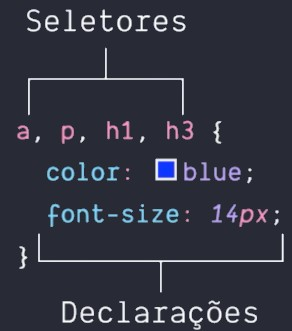
\includegraphics[width=0.3\linewidth]{images/o-que-sao-seletores}
		\caption{O que são seletores (neste exemplo, o seletor é um seletor de tipo).}
		\label{fig:o-que-sao-seletores}
	\end{figure}
	
	ID ou classe podem ser criadas para alterar propriedades de alguns elementos, mesmo que não sejam do mesmo tipo. Dessa forma, pode-se alterar especificamente um elemnto sem modificar os outros elementos do mesmo tipo dentro da página.
	
	\textbf{ID x Classe}: podem representar quaisquer tipos de elementos. No HTML, você declara o seu Id com \textit{id} e sua classe com \textit{class}. No CSS, uma classe é precedida por um ponto e um ID, por um \textit{hash}, como mostrado na Figura \ref{fig:id-x-classe}. Um Id só pode ser usado uma vez na página.
	Exemplo: \textit{<header id="header" class="header"></header>}
	
	\textit{<header id="header" class="header"></header>}

	\begin{figure}[tbph!]
		\centering
		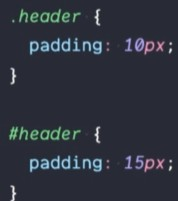
\includegraphics[width=0.3\linewidth]{images/id-classe}
		\caption{ID x CLasse.}
		\label{fig:id-x-classe}
	\end{figure}

	\textbf{Exercício}: Vamos adicionar algumas classes no nosso site e alterar alguns elementos.
	
	\textbf{Obs.:} Para visualizar no navegador o código que gerou a página, basta apertar \textbf{F12}.
	
	\subsubsection{Conceitos básicos}
	
	O navegador representa cada elemento HTML como uma caixa retangular, chamada \textbf{\textit{Box model}}, mostrada na Figura \ref{fig:box-model}. Com o CSS, é possível alterar a aparência dessa caixa. O \textit{Box model} tem quatro áreas:
	
	\begin{description}
		\item[\textit{margin} (margem)] São os espaçamentos entre os elementos.
		\item[\textit{border} (borda)] Circundam o \textit{padding} e o \textit{content}. Pode-se alterar sua largura e cor.
		\item[\textit{padding} (preenchimento)] É o espaçamento entre a \textit{border} e o \textit{content}. 
		\item[\textit{content} (conteúdo)] É o que seu elemento representa, como um texto, uma imagem ou um vídeo.
	\end{description}
	
	\begin{figure}[tbph!]
		\centering
		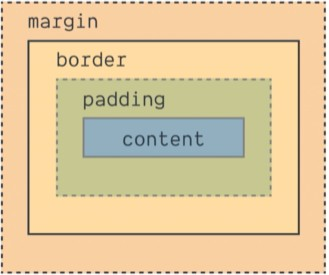
\includegraphics[width=0.3\linewidth]{images/box-model}
		\caption{\textit{Box-model}.}
		\label{fig:box-model}
	\end{figure}

	\textbf{Exercício}: Para enxergarmos o \textit{box model}, vamos adicionar cores e bordas a alguns elementos.
	
	\subsubsection{Material de apoio - CSS3} \label{sec:material-de-apoio-css}
	
	\paragraph{Definição e seletores} \mbox{} \\
	
	Após a criação do HTML a necessidade de formatar as páginas ficou evidente, assim, em 1996, foi criada a linguagem de estilo que conhecemos por CSS.
	
	A sintaxe é bem simples e pode ser explicada com a frase "você cria regras de estilo para elementos ou grupos de elementos".
	
	Vamos usar um elemento HTML que vimos anteriormente, a âncora <a>, para exemplificar.
	
	Uma regra CSS é representada por um seletor ou um grupo de seletores, no nosso caso é o <a>, então dentro de um par de chaves adicionamos as declarações, no exemplo acima estamos alterando cor e tamanho da fonte dessa âncora, as declarações são formadas por uma propriedade e um valor.
	
	Percebam que podemos colocar vários seletores em uma regra separando-os por vírgula.
	
	E há um último detalhe nesse exemplo: a pseudo-classe. Elementos HTML sofrem alterações causadas pela interação do usuário, como mover o mouse por cima ou clicar nesse elemento.
	
	O a:hover do exemplo significa que a âncora também terá essa aparência quando o usuário passar o mouse por cima de um hyperlink.
	
	\paragraph{ID x Classe} \mbox{} \\
	
	No exemplo anterior criamos uma regra que altera um elemento HTML diretamente, mas isso significa que todos os elementos <a> ficarão com aquela aparência, e normalmente temos sites mais complexos que precisam de várias regras diferentes para elementos iguais.
	
	Para ficar mais tangível vamos relembrar um pouco o site que começamos a fazer no módulo passado, ele tinha vários elementos header, mas não vamos querer que o header principal tenha a mesma formatação que o header de uma postagem, é aí que entram os IDs e Classes.
	
	O seletor que vimos no primeiro exemplo é um seletor de tipo, pois ele representa um elemento HTML, e com IDs e Classes podemos representar qualquer tipo de elemento mas há algumas diferenças entre eles:
	
	\begin{description}
		\item[ID] é representado pelo símbolo \# (hash) seguido de um nome para esse ID.
		
		\item[Classe] a classe é representada de forma parecida do ID, mas é precedida por um ponto em vez do hash.
	\end{description} 
	
	E a diferença mais importante entre eles é a forma como devem ser usados: o ID só pode ser usado uma vez em uma página HTML enquanto a classe não tem restrições.
	
	\paragraph{Exercício} \mbox{} \\
	
	Vamos adicionar algumas classes no nosso site e alterar alguns elementos, mas antes precisamos adicionar um arquivo CSS a nossa página.
	
	No módulo de HTML descobrimos que podemos adicionar CSS de duas formas, com o elemento style, e assim suas regras ficarão no arquivo HTML, ou podemos criar um arquivo CSS e adicioná-lo na página através do elemento link, e é essa forma que usaremos.
	
	Crie um elemento link dentro do head do seu arquivo e adicione os atributos rel="stylesheet" e href="style.css", o rel denota o tipo de arquivo que estamos incluindo na página e o href é o caminho para o arquivo. E na mesma pasta do arquivo HTML crie um arquivo chamado style.css.
	
	Agora sim vamos ao CSS, adicione um ID \#title ao h1 da página, pois queremos que ele seja único, e depois adicione as classes .subtitle e .post\_title ao h2 e h3, respectivamente.
	
	No arquivo CSS vamos mudar a cor desses três títulos, e depois alterar o tamanho da fonte do título da postagem.
	
	\paragraph{Box-model} \mbox{} \\
	
	Quando estamos criando o layout de um site o navegador representa cada elemento HTML  como uma caixa retangular, isso é o box-model. E com CSS nós alteramos a aparência dessa caixa (largura, altura, cor de fundo, etc.). Essa caixa é composta por 4 áreas: o conteúdo, o padding, a borda e a margem.
	
	\begin{description}
		\item[margens (margin)] são espaçamentos entre elementos;
		
		\item[bordas (border)]
		
		\item[padding] é um espaçamento entre as bordas e o conteúdo, a diferença para as margens é que declarações de imagem de fundo funcionam nele;
		
		\item[conteúdo (content)] é o que o seu bloco representa, um texto, uma imagem, um vídeo;
		
	\end{description}
	
	\paragraph{Exercício} \mbox{} \\
	
	Para enxergamos o box-model vamos adicionar cores e bordas a alguns elementos.
	
	Primeiro adicionaremos uma cor de fundo para a visualização ficar mais fácil, usaremos a propriedade background com o valor \#fcfcfc no elemento body.
	
	Depois vamos adicionar uma classe ao <article>, pode ser .post, e então vamos colocar a cor branca de fundo com a propriedade background e o valor \#FFF. Agora conseguimos enxergar o content do box-model.
	
	Vamos adicionar um padding de 10 pixels neste mesmo article. Perceberam o espaçamento que surgiu em volta do nosso conteúdo?
	
	Agora adicionamos um borda mais escura a ele com a propriedade border. Vou falar mais detalhadamente sobre border mais a frente, mas por enquanto vamos deixar essa borda com 3 pixels de largura, o contorno sólido e a cor azul.
	
	E por último vamos adicionar uma margem do lado de fora do post com a propriedade margin e o valor 10 pixels.
	
	E agora inspecionando o nosso elemento conseguimos todas aquelas camadas citadas antes: o conteúdo em azul, o padding em verde, as bordas em marrom e as margens em laranja.
	
	E já que começamos a falar sobre bordas e cor de fundo, no próximo vídeo vamos nos aprofundar nessas propriedades.
	
	\paragraph{Estilizando elementos} \mbox{} \\
	
	Agora que entendemos o box-model podemos focar em deixar nosso site mais bonito, então vamos repassar pelas propriedades já citadas:
	
	\begin{description}
		\item[Padding e Margin] Anteriormente usamos o padding e o margin da forma mais básica, com apenas um valor, mas eles são mais poderosos que isso. Se quisermos atribuir tamanhos diferentes para cada lado do box nós podemos, e vamos ver três formas de fazer isso.
		
		A primeira é colocando um valor para as partes superior e inferior e depois para os lados esquerdo e direito.
		
		O valor de 10 pixels se refere ao eixo Y, ou partes superior e inferior, e os 5 pixels se referem aos lados esquerdo e direito.
		
		A segunda forma é dando valores para cada lado do box.
		
		Então começamos pelo topo com 15 pixels, passamos o lado direito com 10 pixels, depois para a parte inferior com 5 pixels e por último o lado esquerdo com 0, e sempre nessa ordem.
		
		Uma boa dica também é que quando o valor for 0 não precisamos não precisamos colocar a unidade.
		
		A terceira forma é com as propriedades específicas para cada lado, até agora tínhamos visto atalhos para essas propriedades.
		
		Essa opção é mais usada quando temos o mesmo valor para 3 lados, e o quarto precisa ter um valor diferente, então usamos o padding com apenas um valor e uma dessas opções para representar o lado diferente.
		
		\item[Background] A propriedade background também é um atalho para várias propriedades, mas isso vocês podem absorver aos poucos, e uma boa opção de leitura é a documentação do MDN Web Docs\footnote{https://developer.mozilla.org/pt-BR/} (\textit{Mozilla Developer Network Web Docs}).
		
		Por enquanto veremos apenas como mudar a cor de fundo.
		
		E aqui temos 3 formas de colocar uma cor de fundo, e ainda existem outras.
		
		A primeira é pelo nome da cor em inglês, a segunda é pelo código hexadecimal e a terceira é usando apenas o atalho background.
		
		\item[Border] Vimos que a propriedade border pode ter 3 valores: a largura (pixels, centímetros, milímetros, ...), a cor (blue, \#0000ff, ...) e o estilo (sólida, pontilhada, tracejada), mas existem algumas particularidades nisso.
		
		A largura pode ser usada com várias unidades, como px, em e mm. A cor pode ser atribuída pelo nome ou por um código hexadecimal, assim como fizemos com o background, e o estilo é representada por palavras-chave, vamos ver algumas delas:
		
		\begin{description}
			\item[solid] Mostra uma borda simples e reta;
			\item[dotted] São bolinhas com um pequeno espaçamento entre elas;
			\item[dashed] Forma uma linha tracejada.
		\end{description}
		
		E aproveitando que mostrei esse código temos que falar sobre como separar a estilização dos lados de uma borda.
		
		E se você não quiser usar a propriedade \textit{border} existem as propriedade específicas para cada aspecto de uma borda, são elas \textit{border-width} para a largura, \textit{border-color} para a cor e b\textit{order-style} para o estilo.
		
		Aqui temos o mesmo código anterior de duas formas diferentes, a primeira com o atalho border e a segunda com cada propriedade específica.
		
		E depois disso podemos juntar os lados com os aspectos de uma borda e criar uma regra mais específica ainda.
		
		\textit{Border-radius} permite arredondar os cantos de um elemento. Podemos usar várias unidades, mas as mais comuns são os pixels e a porcentagem.
		
		Colocando apenas um valor mudamos todos os cantos do elemento, mas seguindo aquela mesma ordem que vimos no \textit{padding} e \textit{margin} - topo, direita, inferior e esquerda - conseguimos alterar cada canto separadamente.
	\end{description}
	
	\paragraph{Exercício} \mbox{} \\
	
	Neste exercício vamos deixar o nosso site um pouco mais bonito usando as propriedades que acabamos de ver.
	
	Vamos aumentar o padding para 15 pixels e colocar uma margem de também de 15 pixels só na parte de baixo do post.
	
	Quando olhamos para os textos percebemos que os espaçamentos estão diferentes do restante do post, então vamos padronizar isso.
	
	No título do post vamos retirar todas as margens para depois colocar apenas uma margem inferior de 15 pixels. E no corpo do post precisamos adicionar uma classe e remover todas as margens para depois adicionar uma margem superior de 15 pixels.
	
	Podemos manter o background branco, mas vamos diminuir a largura das bordas para 2 pixels e mudar a cor para a mesma do texto - \#505050 - e por último adicionaremos um border-radius, 5 pixels são suficientes. Podemos adicionar esse mesmo de valor de border-radius na imagem, para isso vamos acrescentar uma class a imagem antes.
	
	\paragraph{Estilizando textos} \mbox{} \\
	
	Já sabemos que podemos mudar cor e tamanho de algumas fontes, e agora vamos nos aprofundar nisso.
	
	\begin{description}
		\item[\textit{font-family}] Com o \textit{font-family} podemos alterar a fonte dos nossos textos, como uma fonte da internet ou uma que esteja instalada no nosso computador, mas vamos nos ater às fontes seguras, chamadas de \textit{web safe fonts}.
		
		Essas fontes são chamadas assim pois são encontradas em quase todos os sistemas e podem ser usadas sem preocupação.
		
		Ao adicionar duas fontes, a segunda serve como um \textit{backup} para o caso da primeira não funcionar.
		
		\item[\textit{font-size}] O \textit{font-size} nos ajuda a mudar o tamanho do texto, existem algumas unidades de medida para ele mas por enquanto os \textit{pixels} são suficientes para nós.
		
		\item[\textit{font-style}] Usamos o font-style para tornar um texto itálico, na maioria das vezes você usará apenas o valor \textit{italic} para ele, mas se precisar tirar o itálico de um texto você pode usar o valor \textit{normal}. Tem fontes que não suportam o valor \textit{italic}.
		
		\item[\textit{font-weight}] Altera o peso do texto. Para as fontes mais simples, é usual usar \textit{normal} ou \textit{bold} (negrito).
		
		\item[\textit{text-transform}] Transforma o texto entre maiúsculas e minúsculas. O valor \textit{uppercase} coloca todo o texto em caixa alta. O valor \textit{lowercase} coloca todo o texto em caixa baixa. E o \textit{capitalize} coloca todas as primeiras letras de cada palavra em maiúscula.
		
		\item[\textit{text-decoration}] Usado para dar destaque em um texto através de linhas. O valor \textit{underline} coloca uma linha abaixo da palavra, o valor \textit{overline} coloca uma linha acima e o valor \textit{line-through} coloca a linha cortando a palavra.
	\end{description}
	
	\paragraph{Exercício} \mbox{}\\
	
	Vamos fazer algumas mudanças nos nossos textos.
	
	\subsection{Estilizando elementos, textos e listas}
	\subsubsection{Estilizando elementos}
	
	\textbf{\textit{Padding}} e \textbf{\textit{margin}}: Tem como colocar espaçamento diferente para cada lado. Na Figura \ref{fig:espacamento01}, o primeiro valor se refere ao espaçamento dos lados superior e inferior, e o segundo valor, aos lados direito e esquerdo. Na Figura \ref{fig:espacamento02}, cada valor representa um lado, na seguinte ordem: parte superior, direita, parte inferior e esquerda. Quando se tem um valor zero, não é preciso usar uma unidade. Na Figura \ref{fig:espacamento03}, tem-se outra alternativa mais usada quando se quer alterar apenas um lado específico.
	
	\begin{figure}[tbph!]
		\centering
		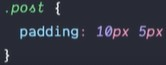
\includegraphics[width=0.3\linewidth]{images/espacamento01}
		\caption{Diferentes espaçamentos para \textit{padding} e \textit{margim}.}
		\label{fig:espacamento01}
	\end{figure}

	\begin{figure}[tbph!]
		\centering
		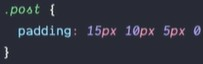
\includegraphics[width=0.3\linewidth]{images/espacamento02}
		\caption{Outra alternativa para diferentes espaçamentos para \textit{padding} e \textit{margim}.}
		\label{fig:espacamento02}
	\end{figure}

	\begin{figure}[tbph!]
		\centering
		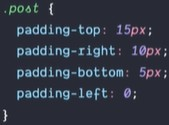
\includegraphics[width=0.3\linewidth]{images/espacamento03}
		\caption{Terceira alternativa para diferentes espaçamentos para \textit{padding} e \textit{margim}.}
		\label{fig:espacamento03}
	\end{figure}
	
	\textbf{Background}:Ttemos 3 formas de colocar uma cor de fundo, e ainda existem outras. A primeira é pelo nome da cor em inglês, a segunda é pelo código hexadecimal e a terceira é usando apenas o atalho background.
	
	\colorbox{red}{Ver material de apoio para essa seção e a seguinte - CSS (Seção \ref{sec:material-de-apoio-css})}
	
	\subsubsection{Estilizando textos}
	
	\subsubsection{Estilizando listas}
	
	\begin{description}
		\item[\textit{list-style-type}] Usado para alterar o marcador de uma lista tanto para uma lista ordenada como para não ordenada.
		
		\item[\textit{list-style-image}] Pode-se usar imagem como marcadores para as listas. Exemplo: \textit{list-style-image: url("rocket.png")} 
	\end{description}

	\textbf{Exercício}: Vamos melhorar a aparência da nossa lista.
	
	\textbf{Obs.:} O CSS funciona como uma cascata. Então pode-se modificar um elemento que esteja dentro do elemento ao qual minha classe ou ID se refere.
	
	\subsection{Dimensão e alinhamento}
	\subsubsection{Propriedades de dimensões e alinhamento}
	
	Propriedades:
	
	\begin{description}
		\item[\textit{Width} e \textit{Height}] Servem para ajustar a largura e a altura de um elemento.
		
		\item[\textit{Max-width} e \textit{Max-height}] Se referem a largura máxima e altura máxima de um elemento.
		
		\item[\textit{Margin}] Coloca espaçamento entre elementos. Tem o valor \textit{auto} que serve para alinhar algum elemento automaticamente.
		
		\item[\textit{Text align}] Serve para alinhar texto.
	\end{description}

	\textbf{Exercício}: Agora vamos delimitar as dimensões dos nossos elementos e alinhar nosso conteúdo.
	
	\section{Recriando a página inicial do Instagram}
	
	Nesse projeto você terá o desafio de reconstruir a página inicial de login do Instagram no qual será abordado o conceito sobre CSS utilizando Flexbox, uma metodologia de posicionamento de elementos em tela mais utilizada no mercado assim como conceitos de responsividade, além disso a expert disponibiliza todo o material necessário em seu GitHub para que você possa realizar o seu projeto.
	
	\subsection{Conteúdos}
	\subsubsection{Como usar os desafios de projetos para cirar seu portifólio}
	
	\subsubsection{Parte 1}
	
	HTML:
	div.nome-da-classe - atalho que cria a divisão
	
	a*2 - Cria duas âncoras
	
	\subsubsection{Parte 2}
	
	CSS: * Selector sleciona todos os elementos
	
	\textit{display: flex;} - Quando usa esse comando em um \textit{container}, ele vira um \textit{flex-container}, ou seja, é um \textit{container} em que todos os elementos que estiverem dentro dele vão ficar em linha ocupando o maior espaço dentro dessa linha
	
	\textit{align-items} - alinha verticalmente. Um dos seus valores é o center.
	
	\textit{justify-items} - alinha horizontalmente. Um dos seus valores é o center.
	
	\subsubsection{Parte 3}
	
	element\textit{.nth-child()} - pega os filhos de um determinado elemento
	
	overflow: hidden; - tudo que extrapolar a bordar não irá aparecer
	
	\subsubsection{Parte 4}
	
	\subsubsection{Objetivo do projeto}
	
	
	\subsection{Informações}
	
	Nesse projeto você terá o desafio de reconstruir a página inicial de login do Instagram, no qual será abordado o conceito sobre CSS utilizando Flexbox, uma metodologia de posicionamento de elementos em tela mais utilizada no mercado assim como conceitos de responsividade, além disso a expert disponibiliza todo o material necessário em seu GitHub para que você possa realizar o seu projeto.
	
	\section{Programação para internet com JavaScript}
	
	JavaScript é uma das mais importantes linguagens front-end, e nesse curso você entenderá o porquê disso e como trabalhar com ela.
	
	\subsection{Introdução ao JavaScript}
	\subsubsection{Introdução ao JavaScript}
	
	\textbf{JavaScript (JS)}
	
	\begin{itemize}
		\item Linguagem de script (execução em tempo real) e multiplataforma;
		\item Client side - é executado do lado do cliente (usuário) - Obs.: quando abre uma página, o navegador executa o JavaScript na sua máquina;
		\item Tem capacidade de interagir com elementos de uma página HTML;
		\item Muito usado no desenvolvimento de páginas e também aplicativos mobile híbridos.
	\end{itemize}

	\textbf{DOM (Document Object Model)} é o documento que o navegador gera quando carrega a sua página, além disso é um modelo de árvore. Por causa disso:
	
	\begin{itemize}
		\item JavaScript pode alterar todos os elementos do HTML;
		\item JavaScript pode alterar todos os atributos e estilos de CSS de uma página.
	\end{itemize}

	Há duas formas do JavaScript interagir no HTML, uma delas é escrevendo o código em JavaScript no \textit{script} dentro do \textit{body}. Ou, usando \textit{script} para referenciar o arquivo do código em JS.
	
	O JS é uma linguagem de tipagem dinâmica. Não precisa dizer o tipo de variável ao declarar, ele identifica o tipo quando é atribuído valor a variável.
	
	Para saber o que está acontecendo no seu programa que está desenvolvendo, usa-se no navegador \textbf{F12} ou botão direito do mouse $\rightarrow$ Inspecionar (Ctrl+Shift+i). Depois vai em \textit{Console}, onde mostra o resultado do \textit{console.log}.
	
	\subsubsection{Array e dicionário}
	
	\subsubsection{Condicionais, laços de repetição e Date}
	
	
	\subsection{Desenvolva páginas web com JavaScript}
	\subsubsection{Desenvolva páginas web com JavaScript}
	
	\subsubsection{Parte 2: Manipulando elementos da página}
	
	
	
	\section{Introdução a Programação com JavaScript (Teste)}
	
	Nesse desafio de codificação você irá praticar através do desenvolvimento de algoritmos os conceitos de pensamento computacional apresentados nas aulas e exercícios anteriores.
	
	\section{Recriando a Interface do Netflix}
	
	Recrie a interface do principal site de streaming mundial utilizando tecnologias simples como HTML5, CSS3 e JavaScript. Nesse projeto você aprenderá: como estruturar o layout, técnicas de CSS3 com containers e variáveis, como posicionar os elementos com Flexbox e como utilizar plugins Jquery a favor da sua aplicação.
	
	\subsubsection{Como usar os desafios de projetos para cirar seu portifólio}
	
	\subsubsection{Parte 1}
	
	\subsubsection{Parte 2}
	
	Extensões no VS Code: 
	
	Live Server  - permite visualizar o navegador a medida que são feitas as alterações no código.
	
	Auto rename tag - com uma alteração no nome da tag de abertura, ele renomeia automaticamente a tag de fechamento e vice-versa.
	
	Dracula Official - muda o tema do VS Code.
	
	html:5 - monta toda a estrutura básica do código em HTML.
	
	Alt+Shift+seta para baixo - clona a linha atual na linha de baixo.
	
	\subsubsection{Parte 3}
	
	\subsubsection{Parte 4}
	
	\subsubsection{Parte 5}
	
	\subsubsection{Parte 6}
	
	\subsubsection{Parte 7}
	
	\subsubsection{Parte 8}
	
	\subsubsection{Parte 9}
	
	\subsection{Informações}
	
	Recrie a interface do principal site de streaming mundial utilizando tecnologias simples como HTML5, CSS3 e JavaScript. Nesse projeto você aprenderá: como estruturar um layout, técnicas de CSS3 com containers e variáveis, como posicionar os elementos com Flexbox e como utilizar plugins Jquery a favor da sua aplicação.
	
	\section{Construindo páginas para internet com Bootstrap}
	
	Aprenda a utilizar o framework Bootstrap e aprofunde mais o seu conhecimento em HTML5 e CSS3.
	
	\subsection{Introdução ao Bootstrap}
	\subsubsection{Aprenda sobre o framework Bootstrap}
	
	\textbf{Bootstrap} (é um framework web com código-fonte aberto para desenvolvimento de componentes de interface e front-end para sites e aplicações web usando HTML, CSS e JavaScript, baseado em modelos de design para a tipografia, melhorando a experiência do usuário em um site amigável e responsivo.): 
	
	\begin{itemize}
		\item Se trata de um framework para desenvolvimento de sites responsivos (são sites que você consegue usar no seu notebook, tablet, smartphone, ..., sem perder a forma);
		\item Possui uma vasta biblioteca de componentes que facilita e agiliza o desenvolvimento de páginas web;
		\item É um dos frameworks mais conhecidos e usados para o desenvolvimento front-end;
	\end{itemize}

	Download Bootstrap: \textcolor{blue}{https://getbootstrap.com/}
	
	Botão direito $\rightarrow$ Exibir código fonte da página (Ctrl+u)
	
	Bootstrap possui as classes \textit{containers}, \textit{row} e \textit{col}. Sempre vai ter uma classe \textit{container}, depois uma classe \textit{row} e, por fim, a classe \textit{col} usada para dividir as colunas. Além disso, divide a página em 12 colunas.
	
	Um arquivo \textit{min} é chamado de minificado, porque o código é aglutinado para reduzir o seu tamanho.
	
	\subsection{Aprenda a utilizar o Bootstrap na sua página WEB}
	\subsubsection{Aprenda a utilizar o Bootstrap na sua página WEB}
	
	Para ver todos os componentes do bootstrap, como os botões: Docs (ou Documentation) $\rightarrow$ Components (lado esquerdo da página).
	
	O bootstrap pode ser visto como um conjunto de estilos para classes e componentes.
	
	Imagens do pexels: \textcolor{blue}{https://www.pexels.com/pt-br/}
	
	\subsection{Crie containers personalizados para o seu site}
	\subsubsection{Crie containers personalizados para o seu site}
	
	Site para código de cores no HTML: \textcolor{blue}{https://htmlcolorcodes.com/}
	
	O \textit{container} cria margens a direita e a esquerda, já o \textit{container-fluid} pega a página inteira. 
	
	Quando há uma cor de fundo é melhor usar o \textit{padding} em vez da \textit{margin} para criar o espaçamento entre os elementos.
	
	\subsection{Trabalhando com imagens dentro de containers}
	\subsubsection{Trabalhando com imagens dentro de containers}
	
	
	\subsection{Crie lista de navegação com imagens em seu projeto}
	\subsubsection{Crie lista de navegação com imagens em seu projeto}
	
	lg - large; md - medium; sm - small
	
	\subsection{Crie lista de navegação dentro de containers utilizando imagens}
	\subsubsection{Crie lista de navegação dentro de containers utilizando imagens}
	
	
	\section{Fundamentos Aritméticos em JavaScript (Teste)}
	
	Nesse desafio de codificação você irá praticar através do desenvolvimento de algoritmos os conceitos de pensamento computacional apresentados nas aulas e exercícios anteriores.
	
	\section{Recriando o jogo da cobrinha com JavaScript}
	
	Já pensou em criar seu próprio jogo do zero? Aprenda a desenvolver de forma simples o clássico jogo da cobrinha utilizando HTML, CSS e JavaScript.
	
	\subsection{Conteúdos}
	\subsubsection{Como usar os desafios de projetos para cirar seu portifólio}
	
	\subsubsection{Parte 1}
	
	\subsubsection{Parte 2}
	
	\subsubsection{Parte 3}
	
	\subsubsection{Parte 4}
	
	\subsubsection{Parte 5}
	
	\subsubsection{Parte 6}
	
	\subsubsection{Objetivo do projeto}
	
	\subsection{Informações}
	
	Já pensou em criar seu próprio jogo do zero? Aprenda a desenvolver de forma simples o clássico jogo da cobrinha utilizando HTML, CSS e JavaScript.
	
\end{document}